\documentclass{report}
\usepackage[english]{babel}
\usepackage[utf8]{inputenc}
\usepackage[T1]{fontenc}
\usepackage[hidelinks]{hyperref}
\usepackage[fixlanguage]{babelbib}
\usepackage{pgfplots}
\pgfplotsset{width=7cm,compat=1.18}
\usepackage{float}
\usepackage{subcaption}
\usepackage{booktabs}
\usepackage{amsmath}
\usepackage{array}
\usepackage{amssymb}
\usepackage{systeme}
\usepackage{tikz}
\usepackage{verbatim}
\usepackage{listings}
\usepackage{lipsum}

\begin{document}

\pagenumbering{gobble}

\begin{titlepage}
    \begin{figure}[!htb]
        \centering
        
\includegraphics[keepaspectratio=true,scale=0.5]{cherubinFrontespizio.eps}
    \end{figure}
    
    \begin{center}
        \LARGE{UNIVERSITÀ DI PISA}
        \vspace{5mm}
        \\ \large{DEPARTMENT OF COMPUTER ENGINEERING}
    \end{center}
    
    \vspace{15mm}
    \begin{center}
        {\LARGE{\bf Edge Computing\\Project Documentation}}
    \end{center}
    \begin{center}
        {
        \makeatletter    
        \@date
        \makeatother    
        }
    \end{center}
    \vspace{30mm}
    
    \begin{minipage}[t]{0.47\textwidth}
        {\large{Team:}{\normalsize\vspace{3mm} \bf\\ \large{Cavedoni F.\\Monaci M.\\Pinna F.}}}
    \end{minipage}
    
    \vspace{15mm}
    \hrulefill
    \\\centering{\large{ACADEMIC YEAR 2024/2025}}
\end{titlepage}

\newpage
\tableofcontents
\newpage

\pagenumbering{arabic}
\setcounter{page}{1}

\chapter{Introduction}

In recent years, the rapid growth of mobile devices and wireless networks has led to a dramatic increase in the demand for efficient and low-latency computational services.
Traditional cloud computing architectures, while powerful, often suffer from latency issues due to the physical distance between end-users and centralized data centers.
To address these challenges, \textit{edge computing} has emerged as a promising paradigm by decentralizing computational resources closer to the users, significantly reducing latency and improving service quality.\\\\
This report focuses on evaluating the performance of a cellular network enhanced with edge computing capabilities. The system under study consists of $M$ base stations arranged in a 2D floorplan of size $L \times H$ according to a regular grid. Each base station is equipped with computational resources and processes user-generated tasks following a \textit{First Come First Served} (FCFS) policy. Additionally, all base stations are interconnected via a mesh topology, allowing communication and task forwarding between them.\\\\
Users are distributed across the floorplan and generate computational tasks at regular intervals. These tasks are sent to the geographically closest base station, which can either process the task locally or forward it to a less-loaded neighboring base station. This introduces a trade-off between processing delays and task-forwarding latency, which depends on the system's load and user distribution.

\section{Problem Description}

We consider $N$ users placed at random locations \texttt{(x, y)} within the same 2D floorplan of size $L \times H$, where the coordinates \texttt{x} and \texttt{y} are random variables to be defined based on specific distributions.
Each user generates a new computational task request every $T$ seconds, and each task consists of $I$ instructions to be executed. Both $T$ and $I$ are exponentially distributed random variables.\\\\
A user sends each new task request to its closest serving base station, which can process the task using one of the following methods:
\begin{itemize}
    \item \textbf{(A)} Serve the request locally at the receiving base station.
    \item \textbf{(B)} Forward the request to the less-loaded base station in the network. If this option is chosen, an additional fixed latency of $D$ milliseconds is added to the total processing time.
\end{itemize}

\section{Objectives}

This project aims to achieve the following objectives:
\begin{itemize}
    \item Evaluate the time required to complete a computing task for various values of $N$, $T$ and $I$, comparing the two methods:
    \begin{itemize}
        \item \textbf{Method (A):} Local task execution at the receiving base station.
        \item \textbf{Method (B):} Task forwarding to the less-loaded base station.
    \end{itemize}
    \item Assess the performance of the system under the following user placement scenarios:
    \begin{itemize}
        \item \textbf{Uniform distribution:} \texttt{x} and \texttt{y} are uniformly distributed random variables in the range:
        \[
        x \in [0, \text{width}], \quad y \in [0, \text{height}]
        \]
        \item \textbf{Lognormal distribution:} \texttt{x} and \texttt{y} follow a lognormal distribution with defined parameters.
    \end{itemize}
\end{itemize}

\section{Performance Metrics}

To evaluate the system's performance, the following metrics are considered:
\begin{itemize}
    \item \textbf{Response time:} The time taken for a task to leave the system after being processed.
    \item \textbf{Queue length:} The number of tasks waiting to be processed at a base station.
    \item \textbf{Packet Dropped:} The number of tasks that are forwarded to an another basestation due to the option B.
    \item \textbf{Packet Dropped:} The number of tasks that are dropped due to insufficient resources.
\end{itemize}
The analysis presented in this report provides insights into the trade-offs and performance implications of local versus collaborative task processing in edge computing-enabled cellular networks. These findings contribute to the understanding and optimization of edge computing architectures for modern applications.

\chapter{Modeling}

\begin{figure}[H]
    \centering
    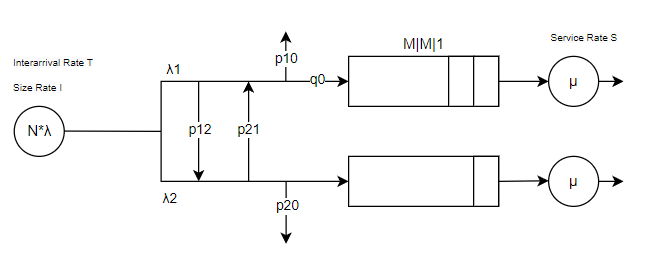
\includegraphics[width=\textwidth]{img/immagine.png}
    \caption{System modeling scheme.}
    \label{scheme}
\end{figure}

The system under study is represented by the scheme shown in \autoref{scheme}. Each base station is modeled as an \texttt{M/M/1/K} queuing system, where $\lambda_i$ represents the arrival rate of tasks at base station $i$, and $\mu$ is the service rate.
Both $\lambda_i$ and $\mu$ are exponentially distributed random variables, which aligns with the Markovian assumptions commonly used in queuing theory. The queues are of finite length, with a maximum capacity of $K$ slots per base station. Any tasks arriving at a base station with a full queue are discarded.\\\\
The system consists of $N$ users generating tasks at an interarrival rate $\lambda$. These tasks are routed to one of the available base stations according to their proximity and load. The system supports task forwarding between base stations, as indicated by the probabilities $p_{ij}$, which represent the likelihood of a task being forwarded from base station $i$ to base station $j$. Forwarding introduces an additional latency, which is assumed to be constant for all base stations.\\\\
As illustrated in the scheme, each task is processed according to a \textit{First Come First Served} (FCFS) policy. The finite queue length $K$ ensures that the system reflects realistic constraints, where resources are limited, and overloading results in task loss. Additionally, tasks may originate from users distributed either uniformly or according to a lognormal distribution, allowing for the evaluation of the system's performance under diverse user distributions.

\section{System Parameters}
Below, we provide a detailed explanation of all the parameters used in the system model, with specific emphasis on their dependencies and characteristics:

\begin{itemize}
    \item \textbf{$N$: Number of users} \\
    The total number of users in the system. These users are distributed across the 2D floorplan according to either a \textit{uniform} or a \textit{lognormal} distribution. Higher values of $N$ result in increased load on the base stations.

    \item \textbf{$K$: Queue length} \\
    The maximum number of tasks a base station can hold in its queue at any given time. If the queue is full, additional incoming tasks are discarded. This parameter models resource constraints at the base station level.

    \item \textbf{$\lambda_i$: Interarrival rate for base station $i$} \\
    The task arrival rate for each base station $i$ depends directly on the user distribution. In the case of a \textit{uniform distribution}, users are evenly spread across the floorplan, leading to nearly balanced $\lambda_i$ values across all base stations. In contrast, for a \textit{lognormal distribution}, certain base stations may experience higher arrival rates due to user clustering in hotspots, resulting in uneven $\lambda_i$ values.

    \item \textbf{$\mu$: Instruction rate (fixed)} \\
    The rate at which instructions are executed at each base station is fixed across the system and represents the computational capacity of the edge servers.

    \item \textbf{Size rate: Packet size distribution (exponential)} \\
    The size of each task (in instructions per packet) follows an \textit{exponential distribution}. This variability in task size directly impacts the service rate for each base station, making it effectively exponential, as the time to serve a task depends on its size.

    \item \textbf{$p_{ij}$: Forwarding probability} \\
    The probability that a task is forwarded from base station $i$ to base station $j$. This depends on the relative load between base stations and is used to balance the computational workload across the system.

    \item \textbf{$D$: Forwarding delay} \\
    The additional latency incurred when a task is forwarded to a less-loaded base station. This delay is assumed to be constant for all tasks and base stations and represents the propagation time in the mesh network.

    \item \textbf{$\mu_{\text{log}}$: Mean of the lognormal distribution} \\
    The mean value of the lognormal distribution used to define the clustering of users in the floorplan. This parameter determines the overall central tendency of user placement in the floorplan.

    \item \textbf{$\sigma_{\text{log}}$: Standard deviation of the lognormal distribution} \\
    The standard deviation of the lognormal distribution, controlling the spread of user placement. Higher values of $\sigma_{\text{log}}$ result in more dispersed user locations, while lower values create tighter clusters.
\end{itemize}

\chapter{Implementation}

The implemented system in OMNeT++ is organized into modular components to reflect the structure and behavior of the edge computing-enabled cellular network. Each module has a specific responsibility, ensuring a clear and maintainable architecture.

\section{Defined Modules}

The following modules have been defined for the simulation:

\begin{itemize}
    \item \textbf{EdgeNetwork (Compound Module)} \\
    This is the top-level module representing the entire system. It hosts the following simple modules:
    \begin{itemize}
        \item \textbf{BaseStation (Simple Module):} Represents a single base station in the network. It is responsible for receiving, processing, and, if necessary, forwarding packets generated by users.
        \item \textbf{User (Simple Module):} Represents a user generating computational tasks. Each user sends packets (with lengths determined by a specified distribution) to its nearest base station.
    \end{itemize}
\end{itemize}

\section{Module Behavior}

The behavior of each module is described in detail below:

\subsection{EdgeNetwork}
\begin{itemize}
    \item Acts as the parent module, hosting all base stations and users within the simulation.
    \item Stores the parameters of all contained modules, allowing them to be retrieved during the simulation using parent pointers.
    \item Provides the spatial layout of base stations and users, ensuring that the correct associations (e.g., nearest base station) are maintained.
\end{itemize}

\subsection{BaseStation}
\begin{itemize}
    \item Receives packets from users in the form of \texttt{cPacket} objects and processes them based on the specified scenario:
    \begin{itemize}
        \item \textbf{Locally Managed:} If the queue has sufficient free slots, the base station enqueues the packet for local processing, ignoring the state of other base stations.
        \item \textbf{Forwarding:} Upon receiving a packet, the base station evaluates the load of all other base stations and forwards the packet to the one with the lowest queue load. If no other base station has a lower load, the packet is processed locally.
    \end{itemize}
    \item Records the following statistics:
    \begin{itemize}
        \item \textbf{Dropped Packets:} The number of packets dropped due to full queues.
        \item \textbf{Forwarded Packets:} The number of packets forwarded to other base stations.
        \item \textbf{Queue Length:} The number of packets in the queue over time, used to compute averages.
        \item \textbf{Response Time:} The time taken for packets to be processed, allowing for average response time computation.
    \end{itemize}
\end{itemize}

\subsection{User}
\begin{itemize}
    \item Generates packets with:
    \begin{itemize}
        \item \textbf{Length:} Packet lengths follow an exponential distribution.
        \item \textbf{Rate:} The packet generation rate also follows an exponential distribution.
    \end{itemize}
    \item Sends each packet to the nearest \texttt{BaseStation}, determined by the Euclidean distance.%
    \footnote{This ensures that users are associated with geographically closest base stations, a common assumption in cellular networks.}
\end{itemize}

\chapter{Verification}
This chapter describes the tests performed to verify the stability and behavior of the system under various scenarios, including extreme and degenerate cases. The results of these simulations help validate the robustness, consistency, and correctness of the implementation.

\section{Degeneracy Test}
This test evaluates the system's stability and behavior under extreme or edge-case conditions. The goal is to ensure that the system remains robust and operates without failures or unexpected behaviors when subjected to these scenarios. By testing the system in degenerate cases, we validate its ability to handle both minimal and excessive loads reliably.

\subsection{Scenario 1 - No Users}
In this degenerate scenario, no users are present in the system. As expected, the system remains stable because there are no packets to process or forward. This verifies the correctness of the system's behavior in edge cases with no load.

\subsection{Scenario 2 - Very High Number of Users}
This scenario tests the system under an extreme load with a very high number of users ($N = 500$) and only two base stations ($M = 4$). 

The system demonstrates robustness under these conditions, maintaining a stable \textit{queue length} and consistent \textit{response time}. The results are shown in \autoref{avg_ql_2} and \autoref{avg_rt_2}, confirming that the system can handle significant load without degenerating.

\begin{figure}[H]
    \centering
    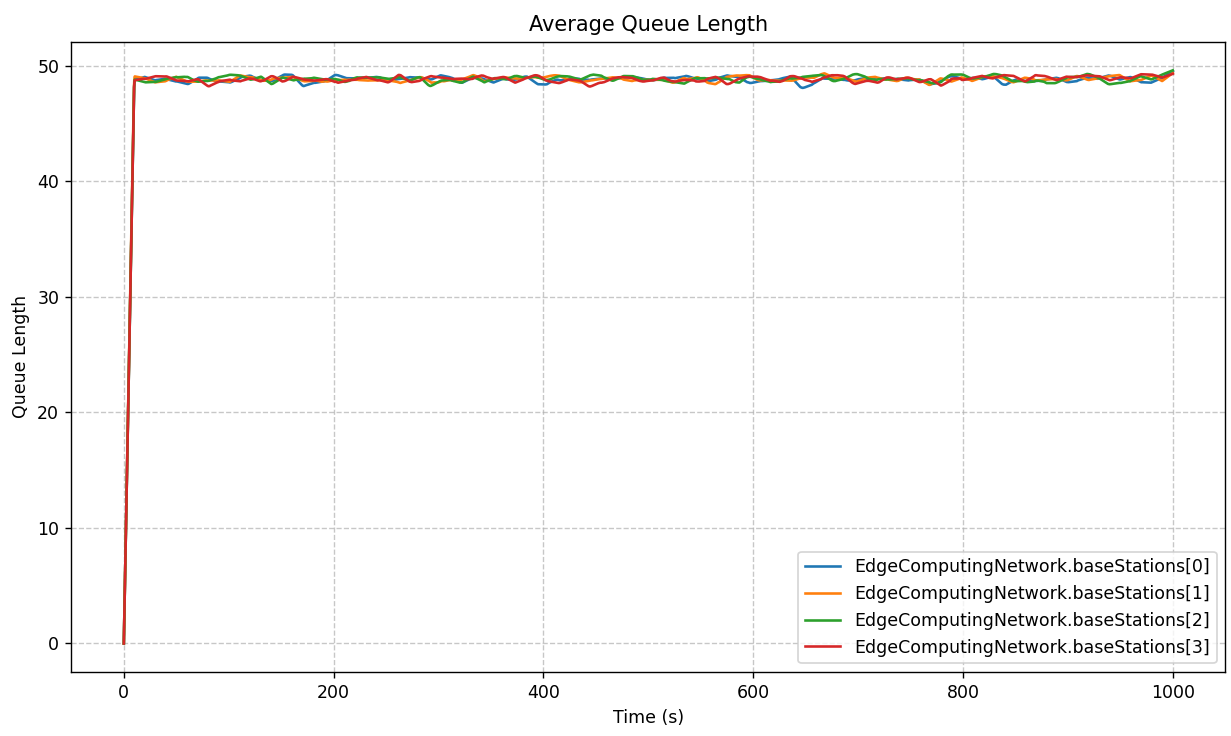
\includegraphics[width=1\textwidth]{img/avg_ql_2.png}
    \caption{Average queue length under high load.}
    \label{avg_ql_2}
\end{figure}

\begin{figure}[H]
    \centering
    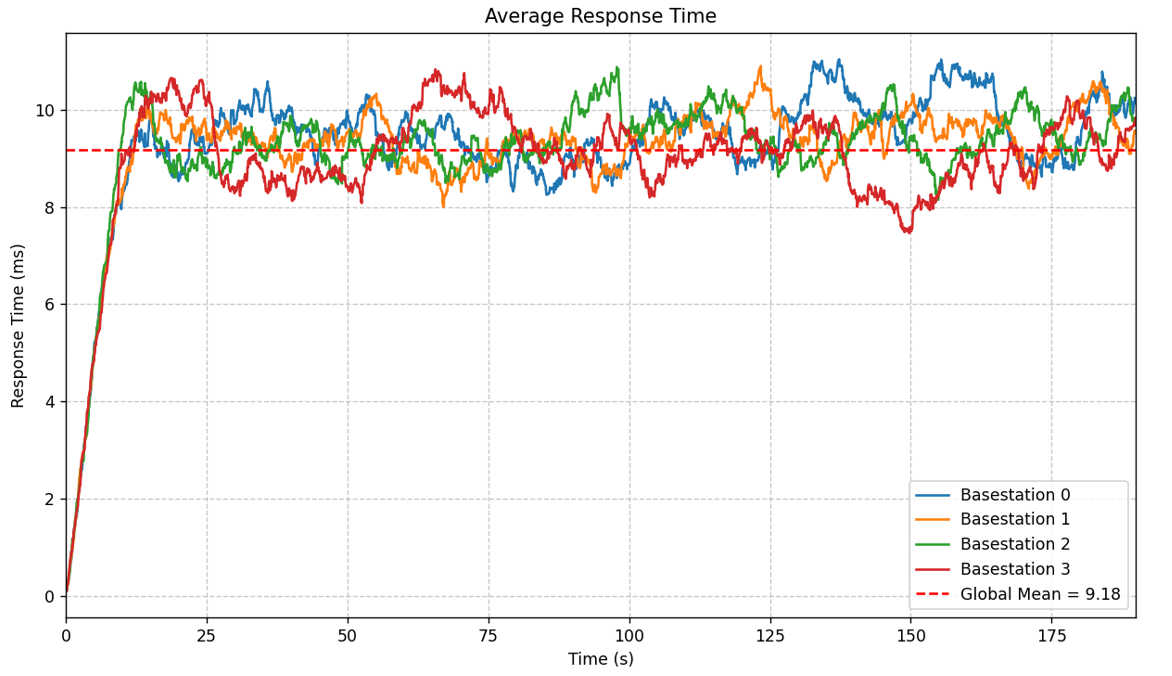
\includegraphics[width=1\textwidth]{img/avg_rt_2.png}
    \caption{Average response time under high load.}
    \label{avg_rt_2}
\end{figure}

\subsection{Scenario 3 - Very Low Service Rate}
This scenario evaluates the system when the service rate is significantly lower than the interarrival rate. \\\\
The simulations show that the queue length stabilizes very fast (\autoref{avg_ql_3}), while the response time exhibits a \textit{linear growth} over time (\autoref{avg_rt_3}). This behavior is consistent with expectations under such extreme conditions.

\begin{figure}[H]
    \centering
    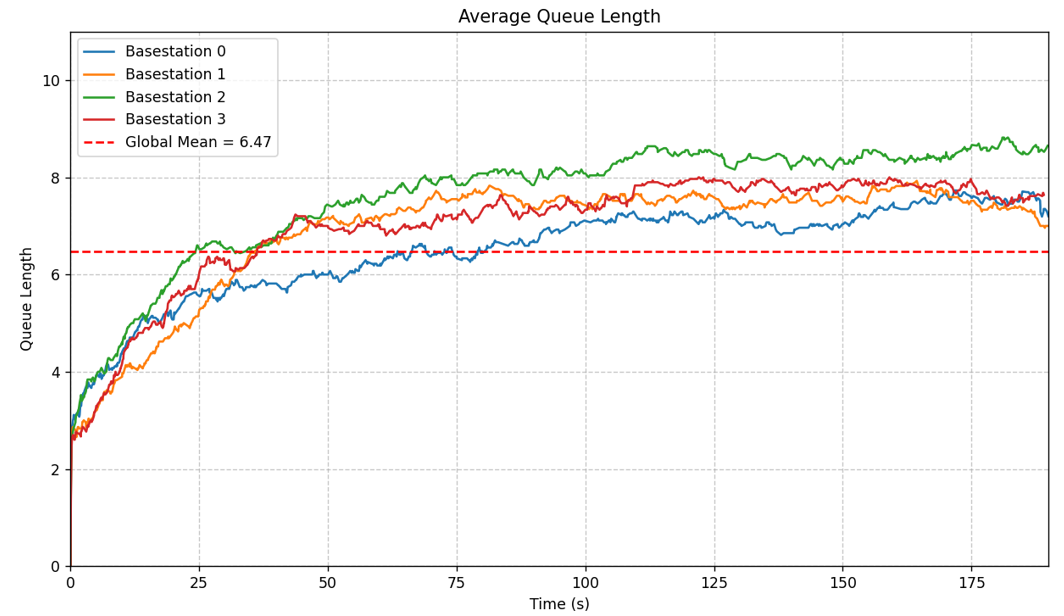
\includegraphics[width=1\textwidth]{img/avg_ql_3.png}
    \caption{Queue length stabilizes under low service rate.}
    \label{avg_ql_3}
\end{figure}

\begin{figure}[H]
    \centering
    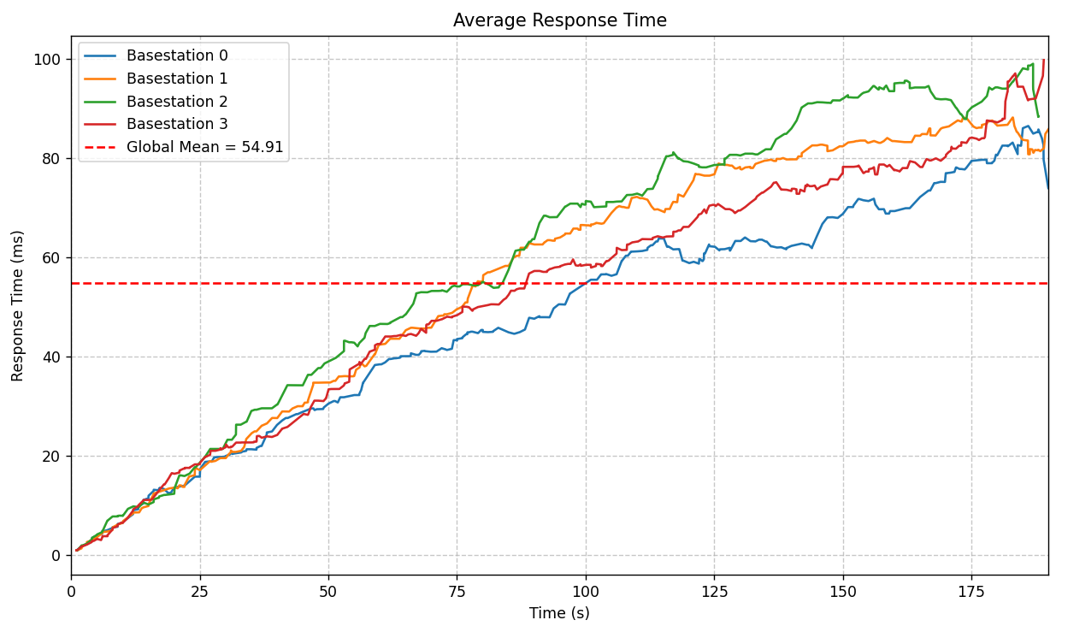
\includegraphics[width=1\textwidth]{img/avg_rt_3.png}
    \caption{Linear growth in response time under low service rate.}
    \label{avg_rt_3}
\end{figure}

\section{Consistency Test}
This test verifies that the system produces coherent results under both configurations: \textit{Locally Managed} and \textit{Forwarding}. \\\\
The results indicate similar mean response times, with the forwarding configuration showing a slight advantage. However, the forwarding configuration also exhibits lower variability, as seen in \autoref{avg_rt_a} and \autoref{avg_rt_b}.

\begin{figure}[H]
    \centering
    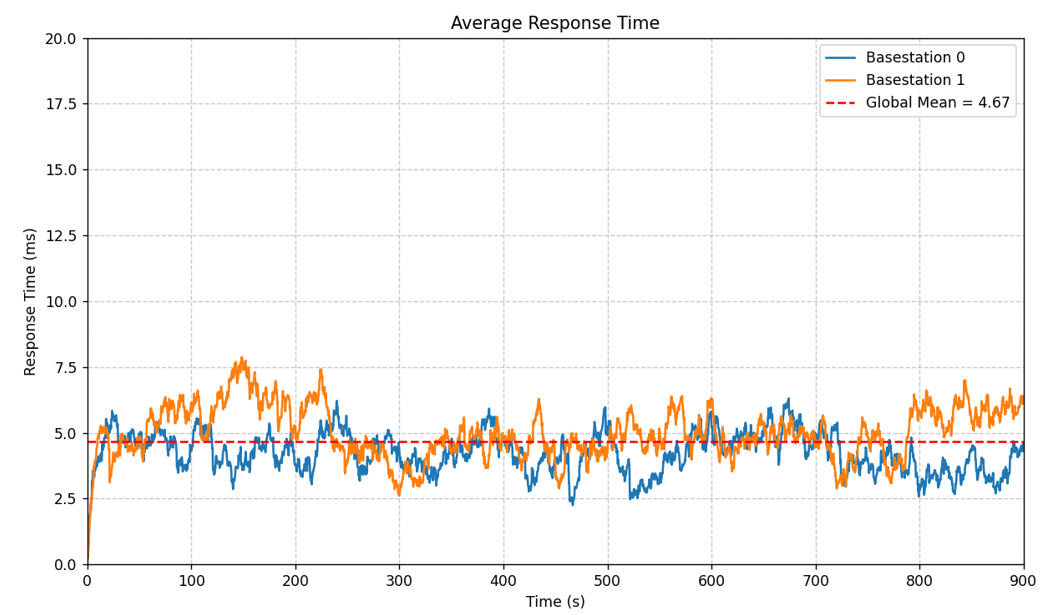
\includegraphics[width=1\textwidth]{img/avg_rt_a.png}
    \caption{Response time: Locally managed.}
    \label{avg_rt_a}
\end{figure}

\begin{figure}[H]
    \centering
    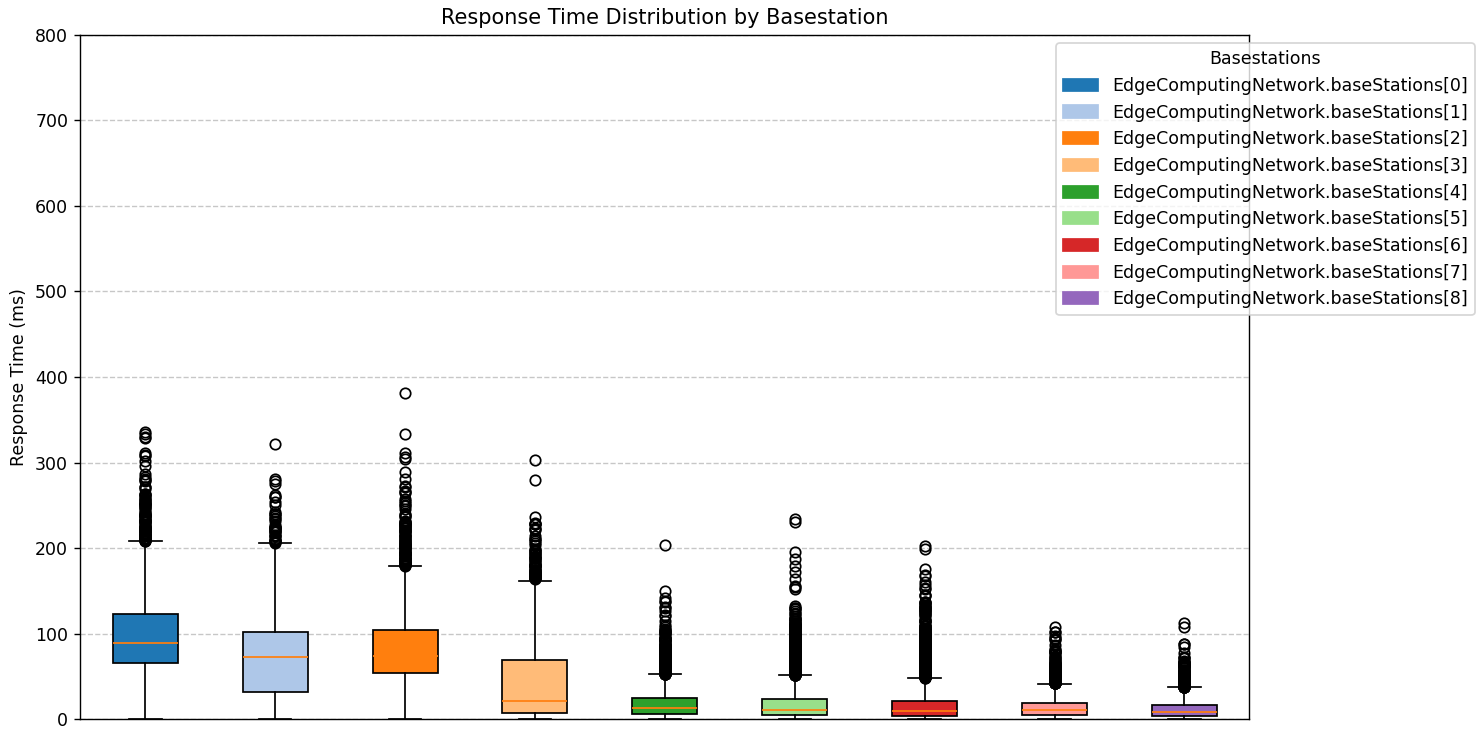
\includegraphics[width=1\textwidth]{img/avg_rt_b.png}
    \caption{Response time: Forwarding.}
    \label{avg_rt_b}
\end{figure}

\section{Continuity Test}
This test ensures that the system responds smoothly when parameters are varied gradually, without abrupt discontinuities in behavior.

\subsection{Increment of Users ($N = 100, 250, 500$)}\label{nusers}
As expected, the mean response time increases with the rising number of users. It remains relatively stable between $N = 100$ and $N = 250$, but exhibits a sharp and significant increase as the number of users reaches $N = 500$.

\begin{figure}[H]
    \centering
    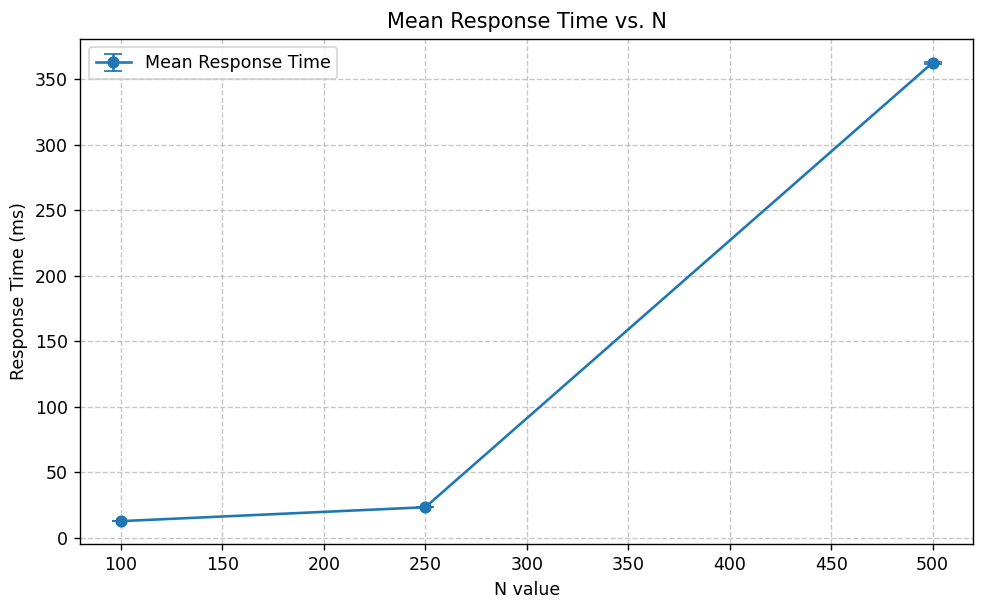
\includegraphics[width=1\textwidth]{img/users_vary.png}
    \caption{Response time for varying numbers of users.}
\end{figure}

\subsection{Increment of Requests' Load ($\lambda = 1/0.1, 1/0.5, 1$)}
At low values of $\lambda$, the mean response time remains relatively low and stable. However, as $\lambda$ approaches $1/0.1$, the mean response time experiences a sharp increase, nearly an order of magnitude higher. This growth is also accompanied by increased variability in the response time.

\begin{figure}[H]
    \centering
    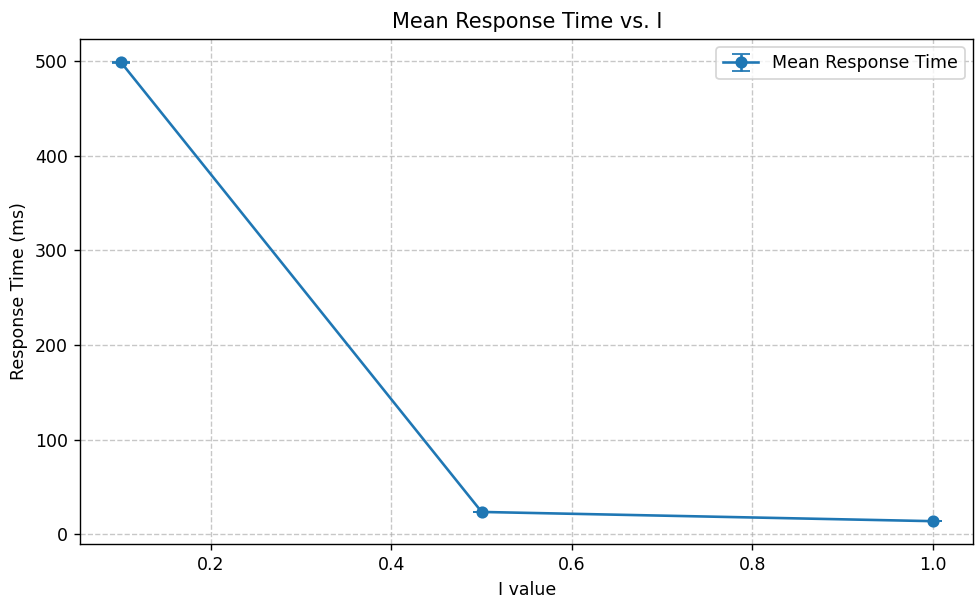
\includegraphics[width=1\textwidth]{img/lambda_vary.png}
    \caption{Response time for varying interarrival rates.}
\end{figure}

\subsection{Increment of Size Rate ($\mu = 100, 1000, 10000$)}
The response time increases significantly as the size rate grows. Notably, for $\mu = 10000$, the response time is two orders of magnitude higher compared to the lower size rates. This trend highlights the strong dependency of response time on the size rate of each packet, as larger packets require substantially more processing time.

\begin{figure}[H]
    \centering
    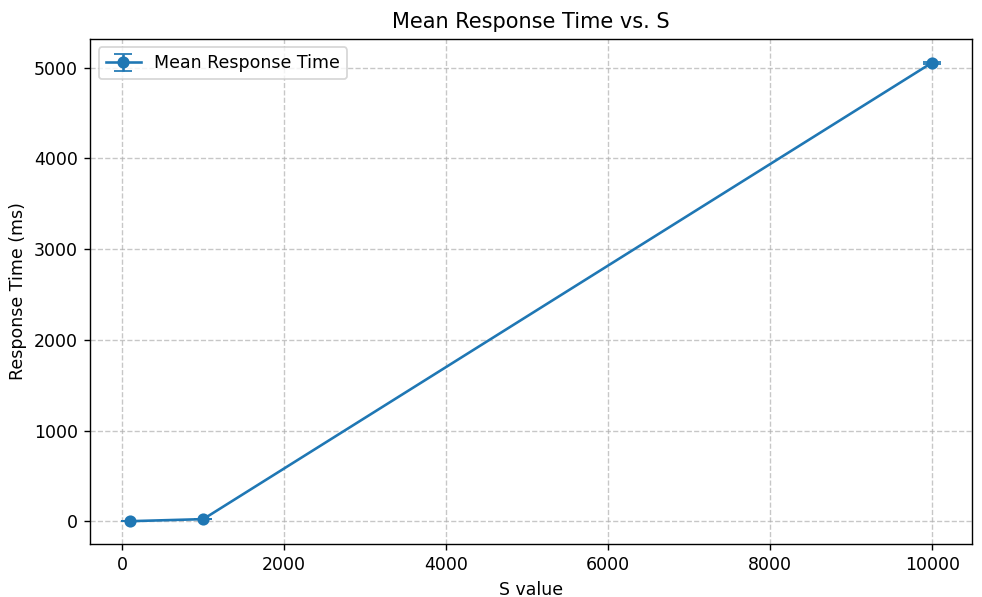
\includegraphics[width=1\textwidth]{img/size_vary.png}
    \caption{Response time for varying service rates.}
\end{figure}

\chapter{Calibration}
In this chapter, we discuss how the factors and parameters have been chosen throughout the development of our system. We distinguish between \textit{fixed factors} and \textit{varying factors} (representing different scenarios).

\section{Factors Calibration}
The objective of this section is to specify the intervals of the key factors in order to correctly reproduce realistic conditions in our system.

\subsection{Fixed Factors}
The following factors remain constant throughout our experiments:

\begin{itemize}
    \item \textbf{Number of base stations (M)}: 9
    %
    \item \textbf{Dimensions of the area}: height = 1800\,m, width = 1800\,m
    %
    \item \textbf{Service rate}: $10^5$ (packets/second)
    %
    \item \textbf{Delay}: 50\,ms
    %
    \item \textbf{Queue size}: 50
    %
    \item \textbf{Distribution parameters}:
    \begin{itemize}
        \item Mean: $\log \left(\frac{1800}{2}\right)$
        \item Standard Deviation: 0.4
    \end{itemize}
\end{itemize}
The number of base stations ($M = 9$) aims to reflect a moderately sized area with multiple sites, balancing suburban and urban deployments. The dimensions of the area ($1800\,m \times 1800\,m$) were chosen to represent a typical environment where base stations are neither too sparse nor too dense. The service rate of $10^5$ packets/second, along with a 50\,ms delay and a queue size of 50, is used to simulate a realistic cellular-network-like environment where moderate buffering and short delays are expected. Finally, the log-normal distribution (characterized by the specified mean and standard deviation) models the spatial distribution of users. This distribution is particularly suitable for analyzing cases where user concentration is uneven across the area, such as in scenarios with hotspots and sparse regions.

\subsection{Varying Factors}
The following factors vary to represent different scenarios and test system performance under varying conditions:

\begin{itemize}
    \item \textbf{Number of users ($N$)}:
    \begin{itemize}
        \item \boldmath{$N = 100$}: Represents a lightly loaded scenario, simulating a low-density environment with fewer active users.
        \item \boldmath{$N = 250$}: A moderately loaded scenario, reflecting a typical environment with a balanced user density.
        \item \boldmath{$N = 500$}: A heavily loaded scenario, used to evaluate system performance under high user density and demand.
    \end{itemize}
    %
    \item \textbf{Interval rate}: This parameter determines how frequently users generate requests (i.e., the arrival rate). We consider two scenarios:
    \begin{itemize}
        \item \textbf{Medium-case scenario}: \boldmath{$1 / 0.5$}, representing a moderate traffic load with steady user activity.
        \item \textbf{Extreme-case scenario}: \boldmath{$1 / 0.1$}, emulating peak traffic conditions with frequent user requests.
    \end{itemize}
    %
    \item \textbf{Size rate}:
    \begin{itemize}
        \item \textbf{Medium-case scenario}: \boldmath{$10^3$}: Corresponds to smaller data packet sizes, typical of lightweight applications or systems with low bandwidth requirements.
        \item \textbf{Extreme-case scenario}: \boldmath{$10^4$}: Represents larger data packet sizes, increasing system load and reflecting heavier traffic conditions.
    \end{itemize}
\end{itemize}
The combination of these parameters enables us to evaluate the system under a broad range of realistic conditions, from moderate loads with fewer users and smaller data sizes to extreme loads with higher user counts, larger data sizes, and higher arrival rates. These variations ensure that the analysis is comprehensive and captures critical performance metrics under both typical and challenging conditions.

\section{Warmup Time Analysis}
Warmup time refers to the period during which the system transitions from an initial transient state to a steady state. Properly setting the warmup time ensures that the system's performance metrics are evaluated only during the steady-state period, avoiding bias caused by the initial transient.\\\\
In our analysis, we observed the response time as a function of time. As shown in Figure~\ref{fig:warmup_time}, the response time stabilizes and reaches a steady state within 100 seconds. The transient period, characterized by larger variations in response time, does not exceed 100 seconds across all experiments.\\\\
Based on these observations, the warmup time is empirically set to 100 seconds. This ensures that any data collected during the transient state is excluded from the analysis, leading to more accurate and reliable results.

\begin{figure}[h!]
    \centering
    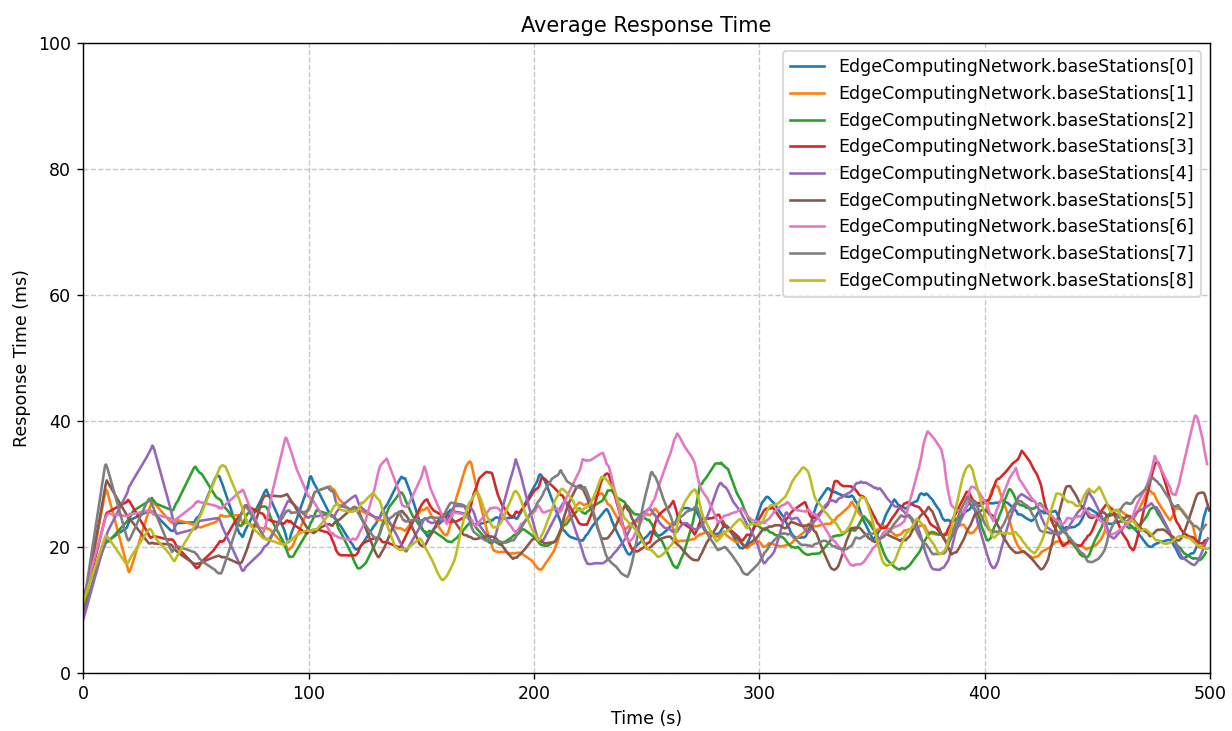
\includegraphics[width=1\textwidth]{img/warmup_analysis.png}
    \caption{Response time as a function of time. The transient period does not exceed 100 seconds, indicating the warmup time.}
    \label{fig:warmup_time}
\end{figure}

\chapter{Simulation Experiments}
\section{The effect of forwarding packets on the system}
We test our system in both cases A and B to see the effects of forwarding packets wether the packets are generated acording to a uniform distribution or a lognormal distribution.\\\\
The tests also take into account 3 factors:
\begin{itemize}
    \item \textbf{N}: (100, 250, 500)
    \item \textbf{Interarrival rate}: ($\frac{1}{0.1}$, $\frac{1}{0.5}$)
    \item \textbf{Size rate}: ($\frac{1}{10^3}$, $\frac{1}{10^4}$)
\end{itemize}

Considering the average case as a reference:
\begin{itemize}
    \item $N=250$
    \item $I=\frac{1}{0.5}$
    \item $S=\frac{1}{10^3}$
\end{itemize}

\subsection{Size rate variation - Method A}
\subsubsection*{Case $S=\frac{1}{10^3}$}

\begin{figure}[H]
    \centering
    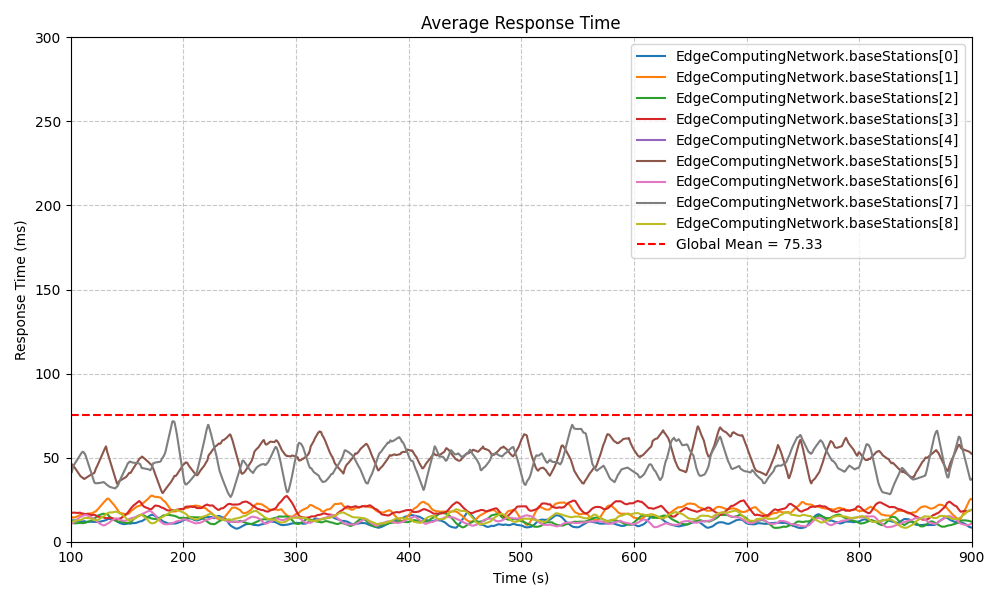
\includegraphics[width=\textwidth]{img/plots/log_1e3_A/resptime.png}
    \caption{$E[R]$ for the lognormal distribution}
\end{figure}

\begin{figure}[H]
    \centering
    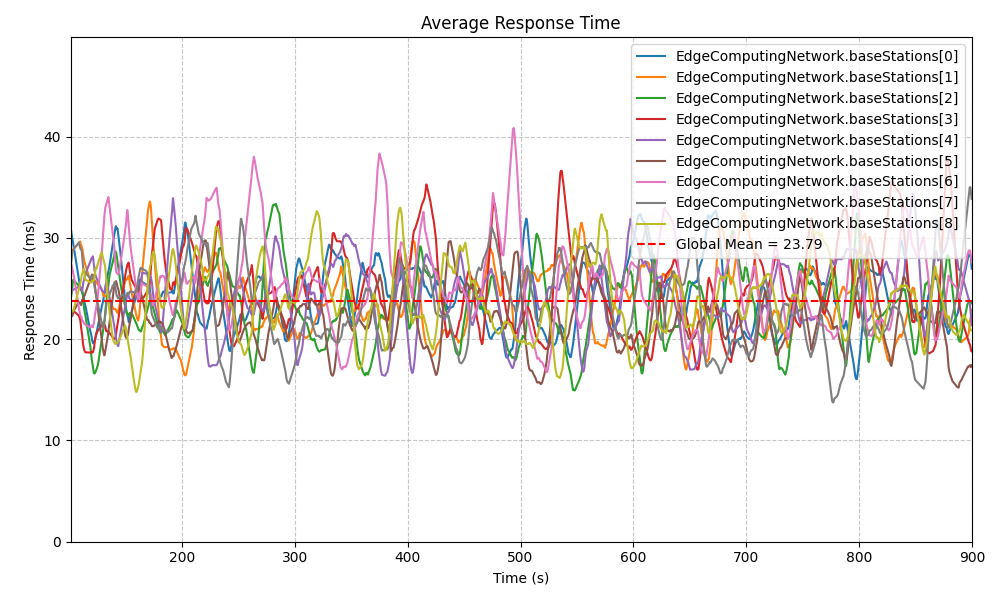
\includegraphics[width=\textwidth]{img/plots/uni_1e3_A/resptime.png}
    \caption{$E[R]$ for the uniform distribution}
\end{figure}

The difference between the two distribution is remarkable, as in the lognormal case we find a higher mean response time and queue length.

\begin{figure}[H]
    \centering
    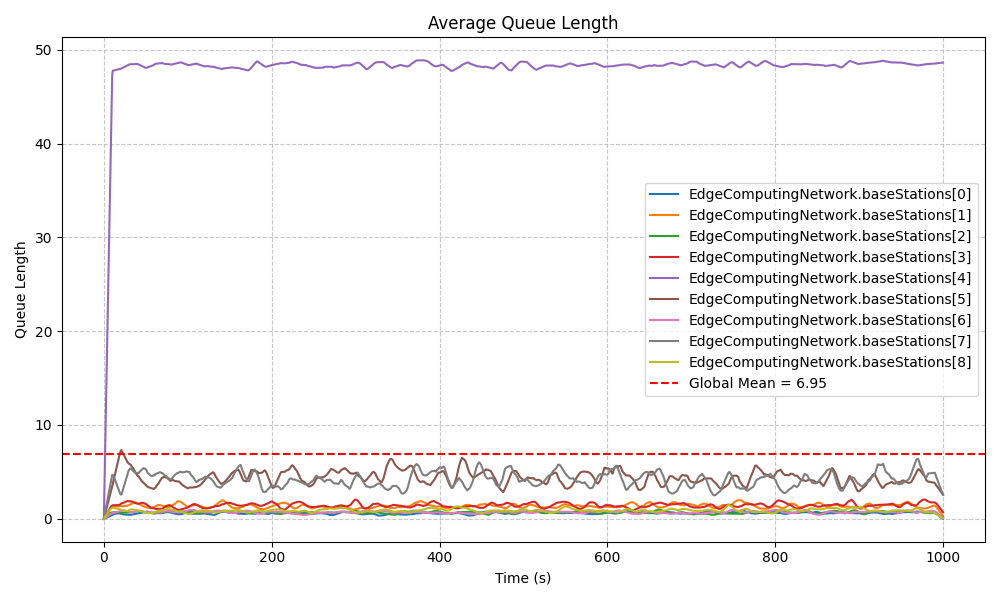
\includegraphics[width=\textwidth]{img/plots/log_1e3_A/qlen.png}
    \caption{$E[qlen]$ for the lognormal distribution}
\end{figure}

\begin{figure}[H]
    \centering
    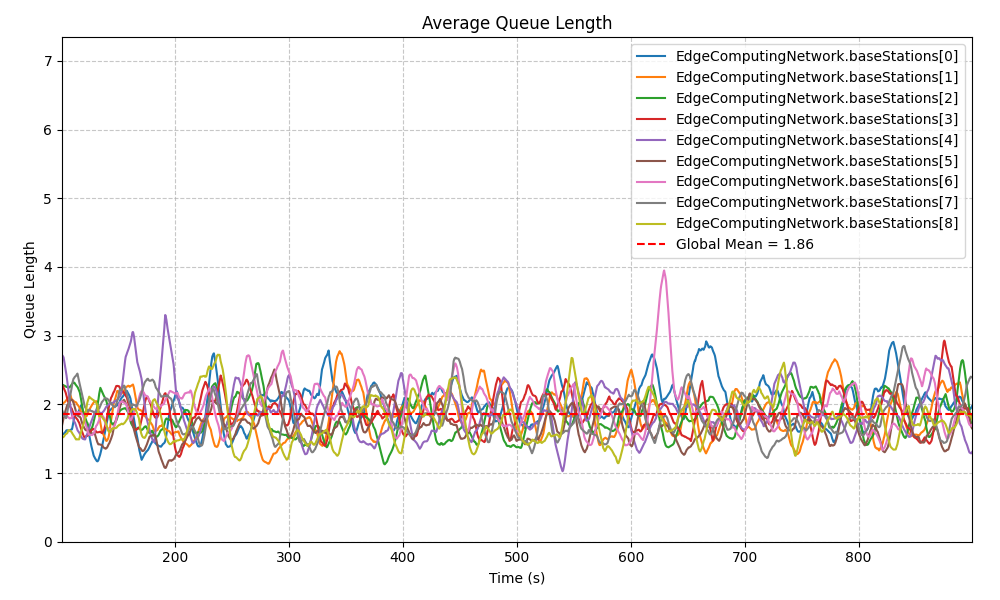
\includegraphics[width=\textwidth]{img/plots/uni_1e3_A/qlen.png}
    \caption{$E[qlen]$ for the uniform distribution}
\end{figure}

In the uniform distribution the values are more compact around the mean, unlike the lognormal case, where is evident that there are one or more base stations dealing with a heavier load.

\begin{figure}[H]
    \centering
    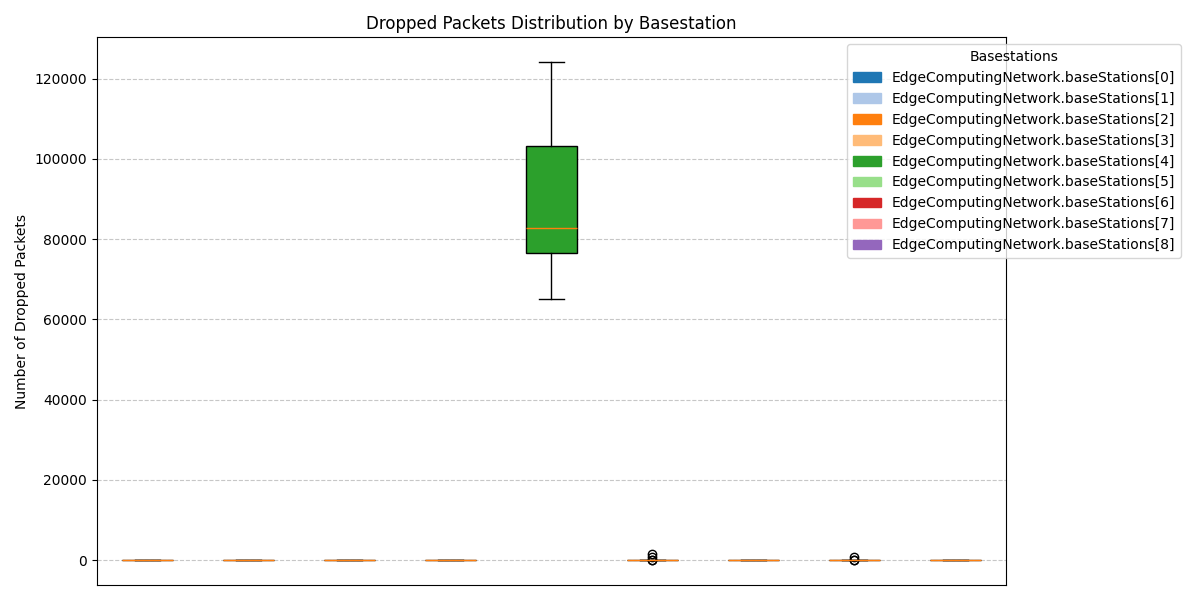
\includegraphics[width=\textwidth]{img/plots/log_1e3_A/dropped.png}
    \caption{Dropped packets distribution (lognormal)}
\end{figure}

\begin{figure}[H]
    \centering
    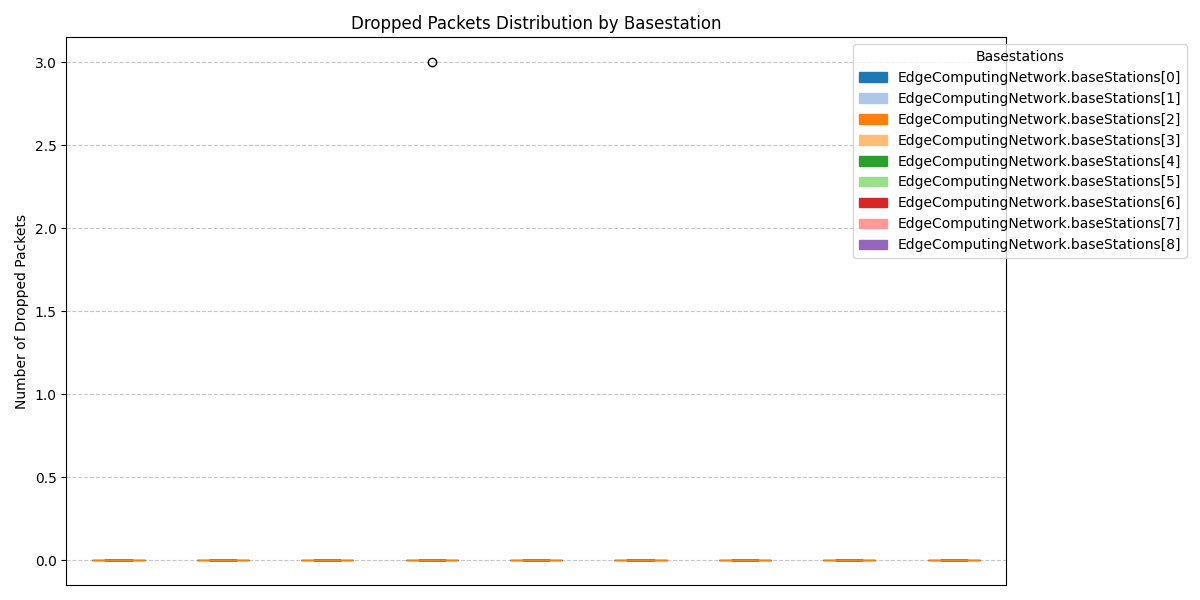
\includegraphics[width=\textwidth]{img/plots/uni_1e3_A/dropped.png}
    \caption{Dropped packets distribution (uniform)}
\end{figure}

\begin{flushleft}
Since base stations use the policy where packets are served locally, a higher queue length might mean a higher number of discarded packets. Even though, the system can still sustain the load in the uniform case as the number of discarded packets is lower than $10$.

\vspace{1em} 

Not the same for the lognormal case, where the total of discarded packets is over $2.5\times10^5$ units.
\end{flushleft}

\vspace{10mm}

\subsubsection*{Case $S=\frac{1}{10^4}$}

\begin{figure}[H]
    \centering
    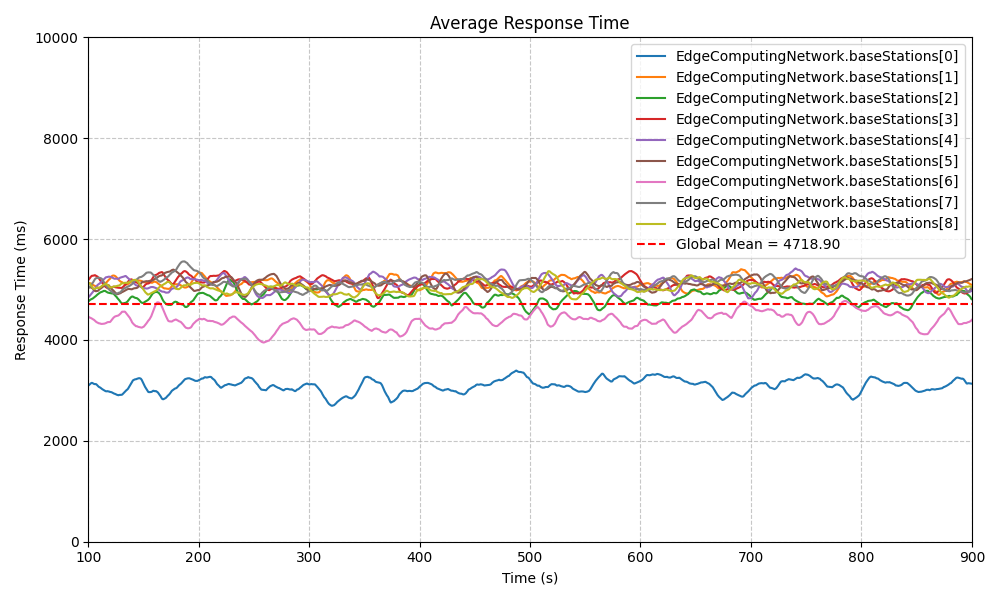
\includegraphics[width=\textwidth]{img/plots/log_1e4_A/resptime.png}
    \caption{$E[R]$ for the lognormal distribution}
\end{figure}

\begin{figure}[H]
    \centering
    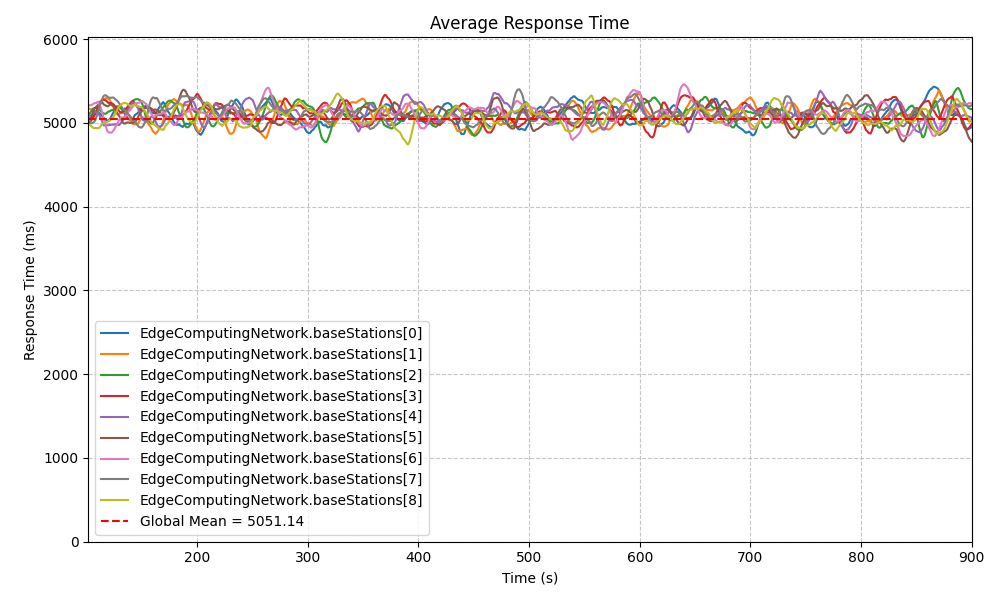
\includegraphics[width=\textwidth]{img/plots/uni_1e4_A/resptime.png}
    \caption{$E[R]$ for the uniform distribution}
\end{figure}

\begin{figure}[H]
    \centering
    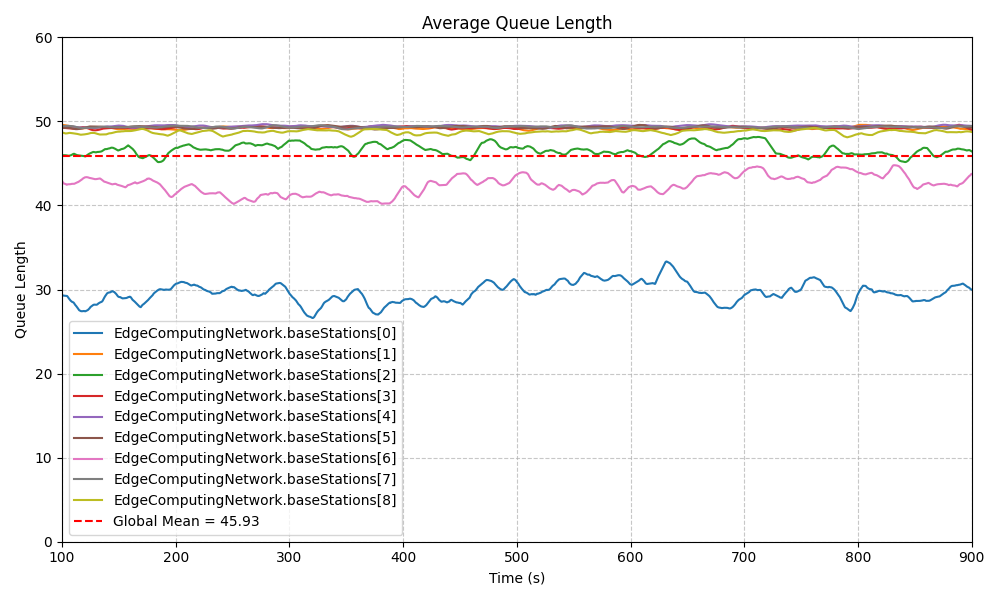
\includegraphics[width=\textwidth]{img/plots/log_1e4_A/qlen.png}
    \caption{$E[qlen]$ for the lognormal distribution}
\end{figure}

\begin{figure}[H]
    \centering
    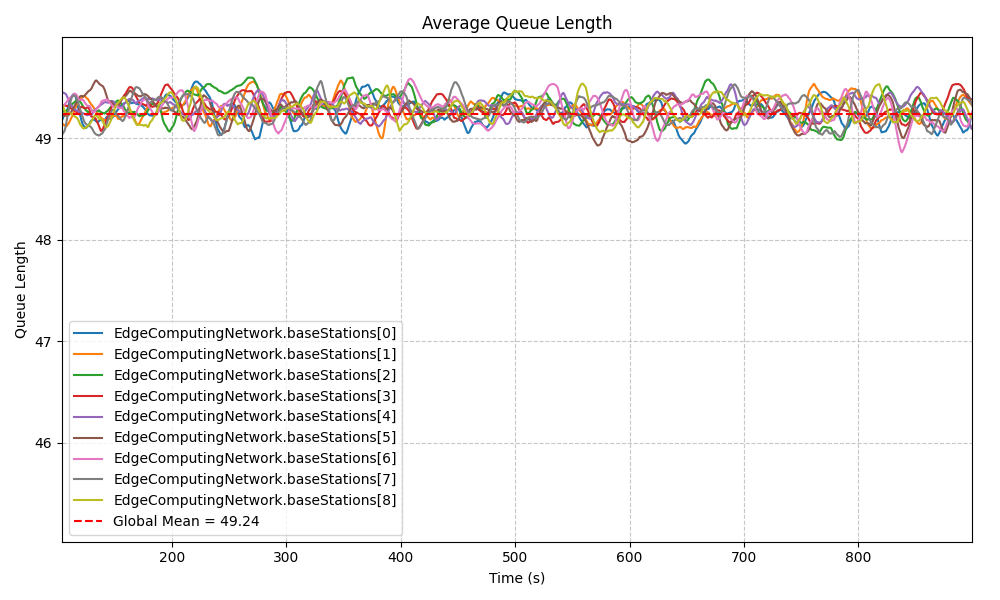
\includegraphics[width=\textwidth]{img/plots/uni_1e4_A/qlen.png}
    \caption{$E[qlen]$ for the uniform distribution}
\end{figure}

This experiment shows how the system can better sustain the load in the lognormal case dealing with bigger packets. Unlike the previous experiment, this time we find similar behaviours.

\begin{figure}[H]
    \centering
    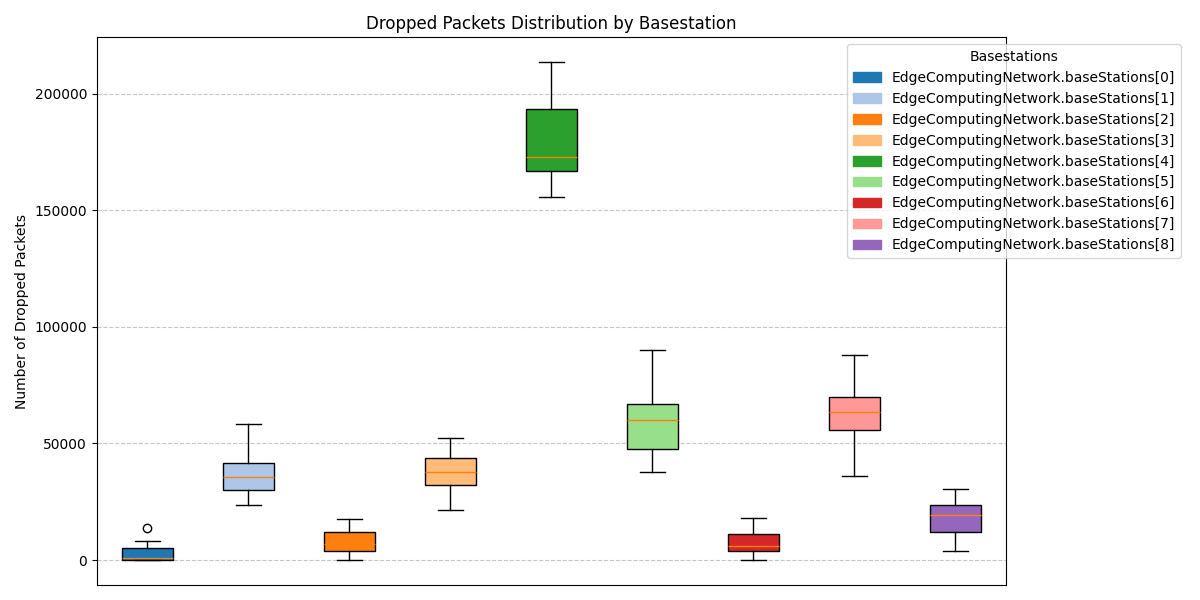
\includegraphics[width=\textwidth]{img/plots/log_1e4_A/dropped.png}
    \caption{Dropped packets distribution (lognormal)}
\end{figure}

\begin{figure}[H]
    \centering
    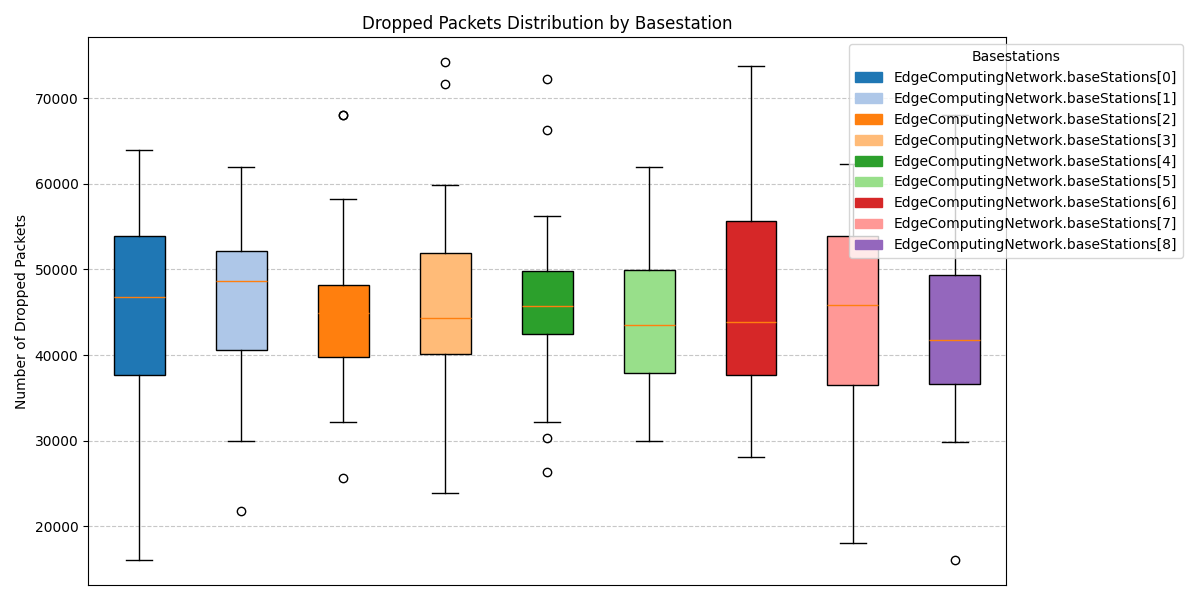
\includegraphics[width=\textwidth]{img/plots/uni_1e4_A/dropped.png}
    \caption{Dropped packets distribution (uniform)}
\end{figure}

\begin{flushleft}
Also the distribution of dropped packets is similar, presenting more concentrated values in the lognormal case.
\end{flushleft}

\subsection{Size rate variation - Method B}
\subsubsection*{Case $S=\frac{1}{10^3}$}

\begin{figure}[H]
    \centering
    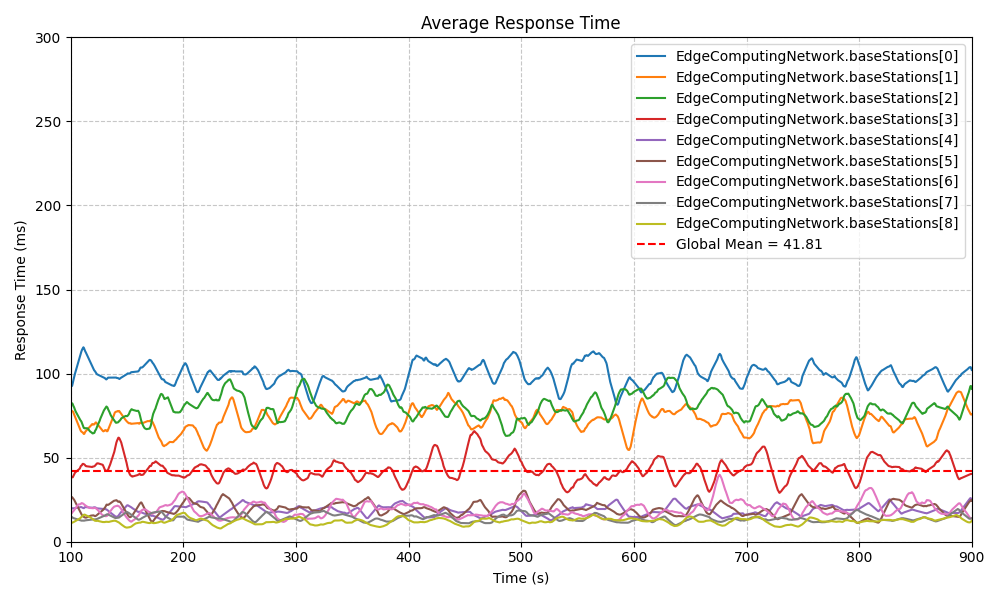
\includegraphics[width=\textwidth]{img/plots/log_1e3_B/resptime.png}
    \caption{$E[R]$ for the lognormal distribution}
\end{figure}

\begin{figure}[H]
    \centering
    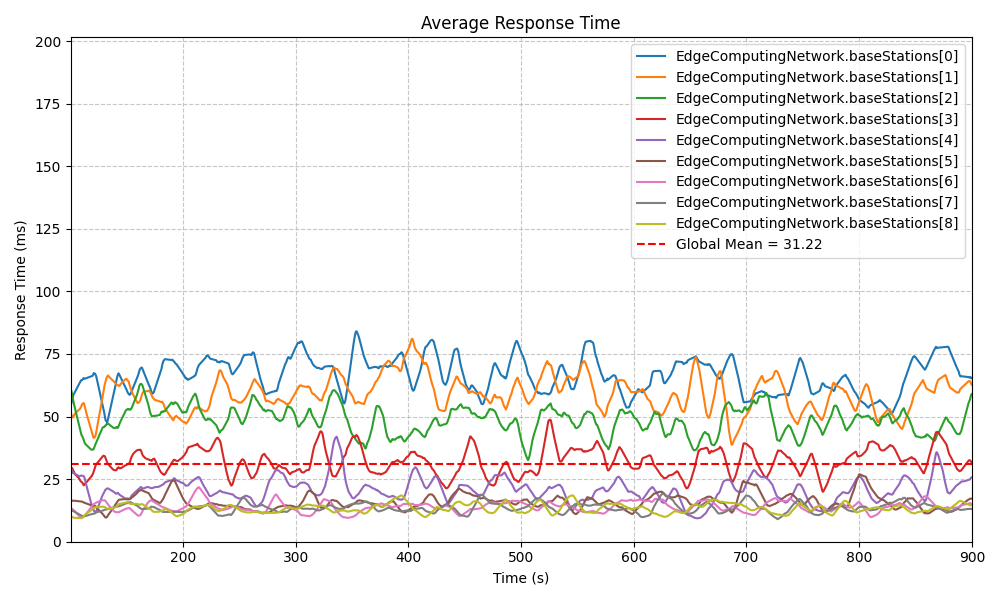
\includegraphics[width=\textwidth]{img/plots/uni_1e3_B/resptime.png}
    \caption{$E[R]$ for the uniform distribution}
\end{figure}

As we can see the performance of the system improves with respect to the method A, but only when dealing with the lognormal distribution. The mean response time in the uniform case gets higher due to the forwarding directed to the same couple of base stations, this behaviour is responsible to raise the mean response time.

\begin{figure}[H]
    \centering
    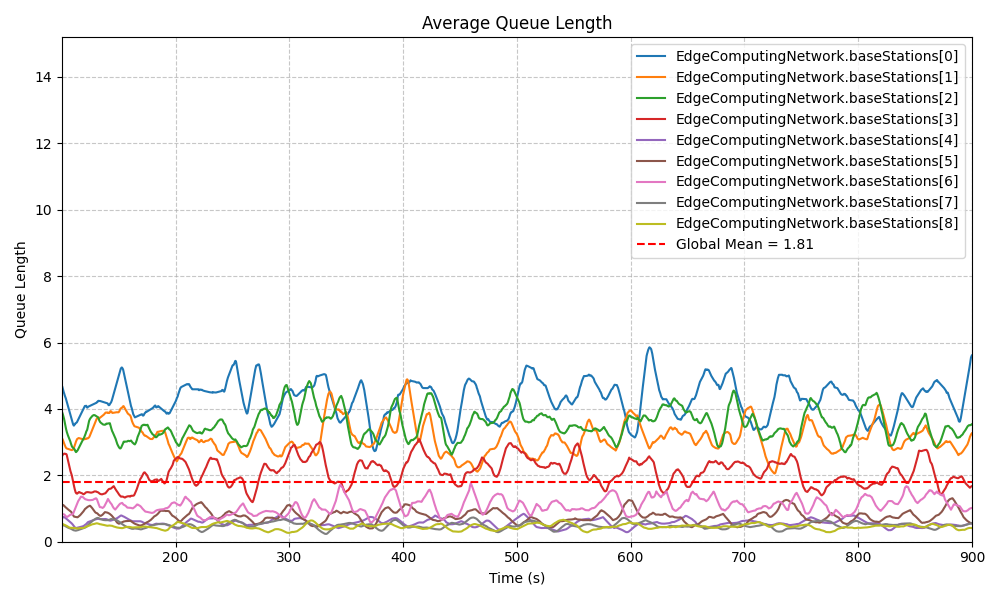
\includegraphics[width=\textwidth]{img/plots/log_1e3_B/qlen.png}
    \caption{$E[qlen]$ for the lognormal distribution}
\end{figure}

\begin{figure}[H]
    \centering
    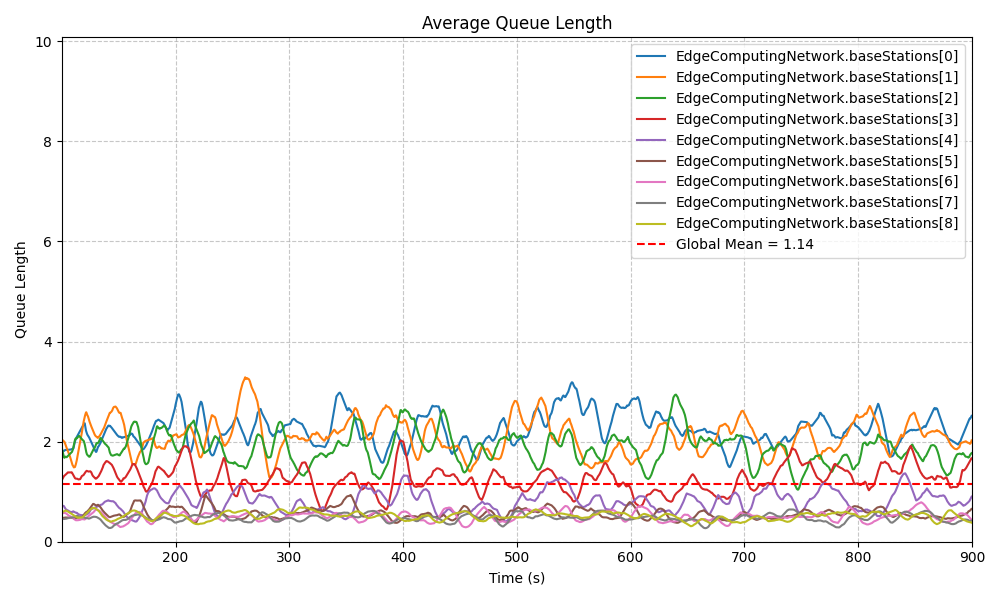
\includegraphics[width=\textwidth]{img/plots/uni_1e3_B/qlen.png}
    \caption{$E[qlen]$ for the uniform distribution}
\end{figure}


\begin{flushleft}
The same reasoning can be applied to the mean leangth of each queue, as the plots show the exact same behaviour.
\end{flushleft}

\begin{figure}[H]
    \centering
    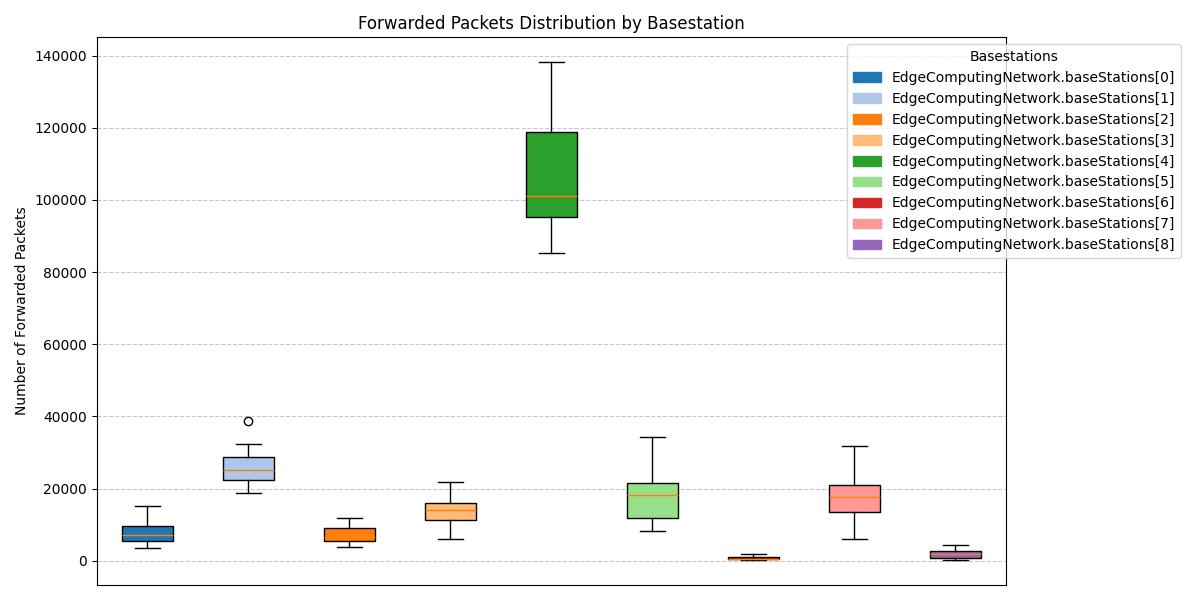
\includegraphics[width=\textwidth]{img/plots/log_1e3_B/forwarded.png}
    \caption{Forwarded packets distribution (lognormal)}
\end{figure}

\begin{figure}[H]
    \centering
    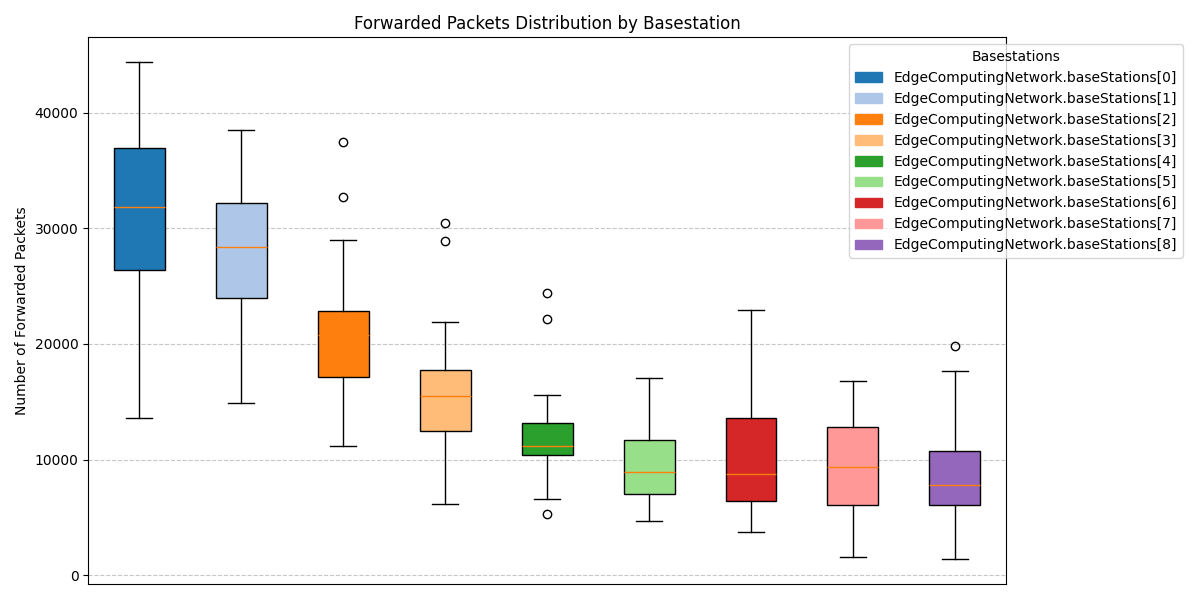
\includegraphics[width=\textwidth]{img/plots/uni_1e3_B/forwarded.png}
    \caption{Forwarded packets distribution (uniform)}
\end{figure}

\begin{flushleft}
It is curious that in the lognormal case packets tend to be forwarded to one particular base station unlike the uniform case, where are forwarded more evenly. The lognormal case presents a higher number of forwarded packets ($5.9\times10^6$ vs $4.3\times10^6$).
\vspace{1em}

Dropped packets are not mentioned as there has been none throughout the experiment.
\end{flushleft}
% LOG
% Total Dropped Packets: 0
% Total Forwarded Packets: 5959327
% UNI
% Total Dropped Packets: 0
% Total Forwarded Packets: 4390846

\subsubsection*{Case $S=\frac{1}{10^4}$}

\begin{figure}[H]
    \centering
    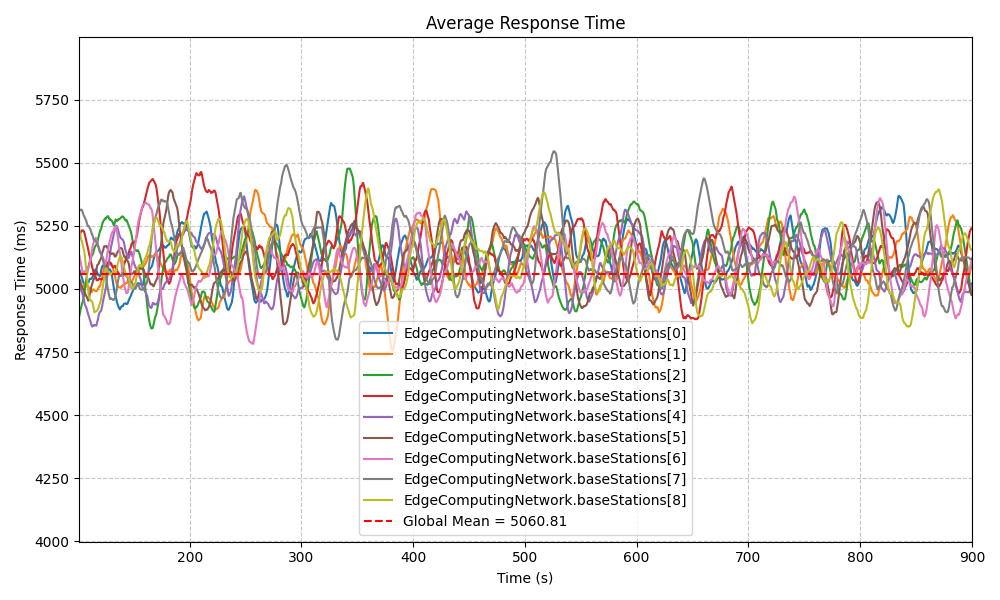
\includegraphics[width=\textwidth]{img/plots/log_1e4_B/resptime.png}
    \caption{$E[R]$ for the lognormal distribution}
\end{figure}

\begin{figure}[H]
    \centering
    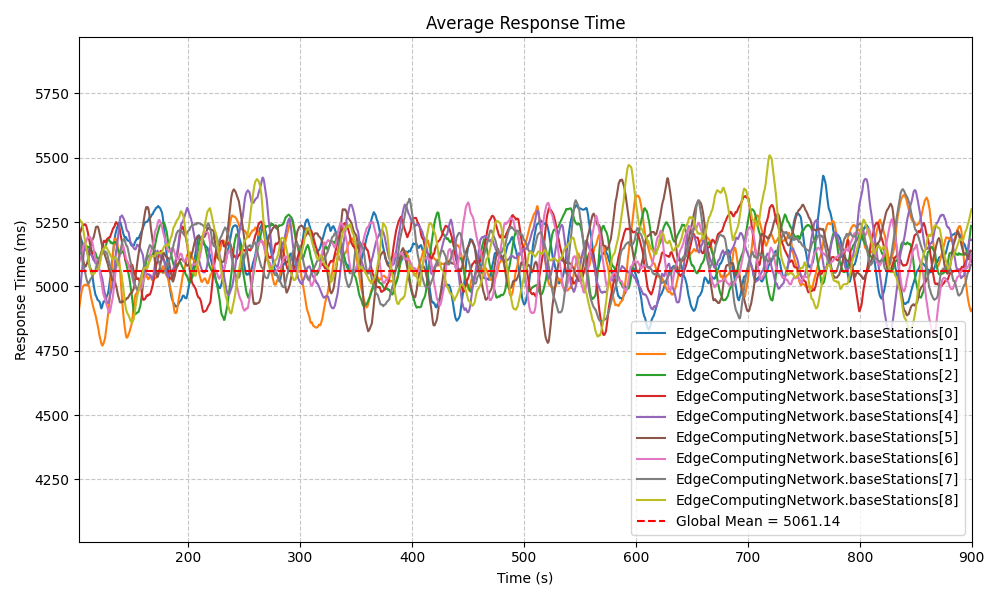
\includegraphics[width=\textwidth]{img/plots/uni_1e4_B/resptime.png}
    \caption{$E[R]$ for the uniform distribution}
\end{figure}

In this case it is cear that the system is stressed out in both the distribution with almost equal mean response time. All the values of the base stations are concentrated around the global mean, which represents the fact that all of them respond at almost the same speed.

\begin{figure}[H]
    \centering
    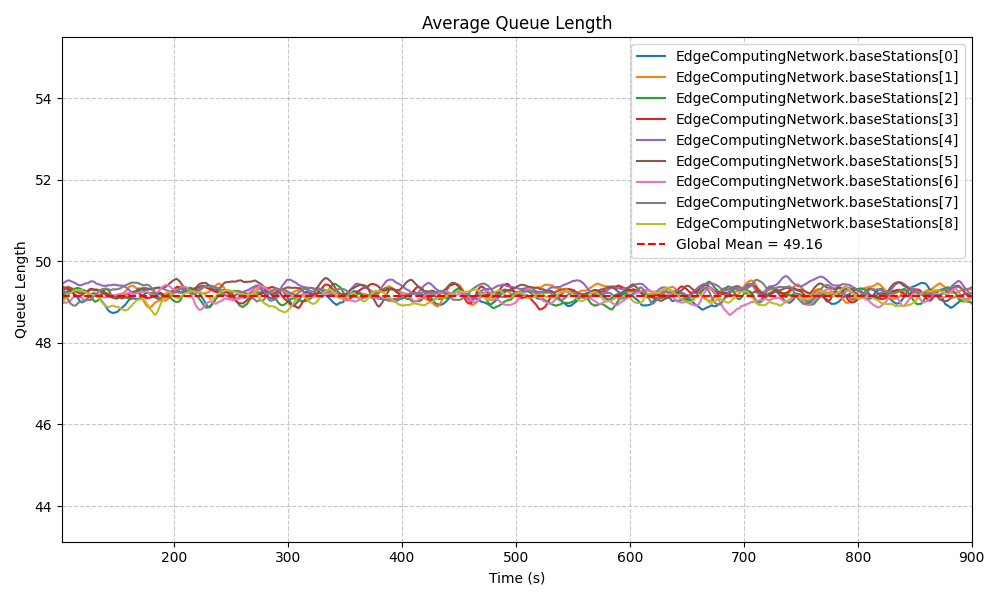
\includegraphics[width=\textwidth]{img/plots/log_1e4_B/qlen.png}
    \caption{$E[qlen]$ for the lognormal distribution}
\end{figure}

% \begin{figure}[H]
%     \centering
%     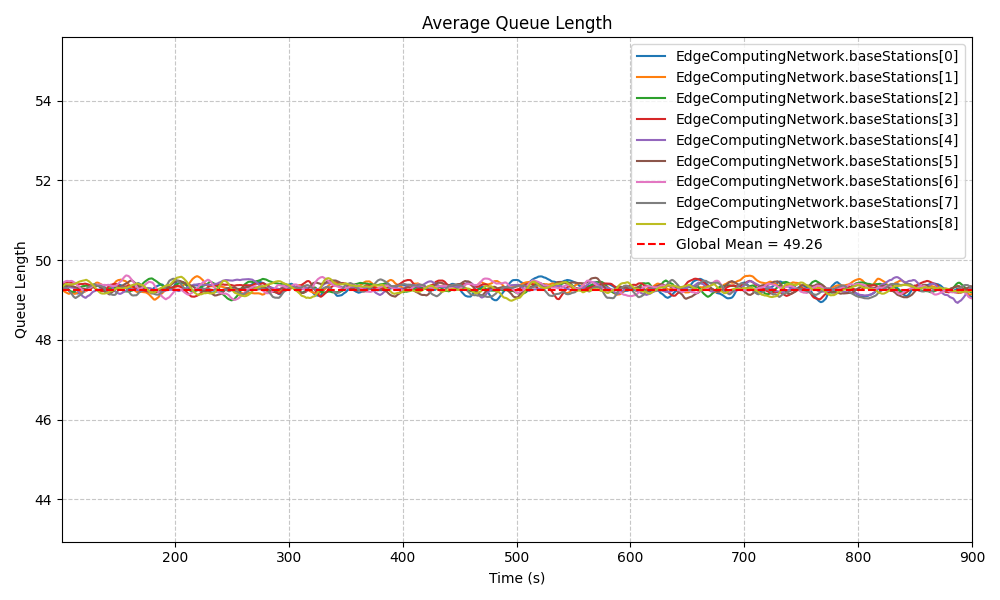
\includegraphics[width=\textwidth]{img/plots/uni_1e4_B/qlen.png}
%     \caption{$E[qlen]$ for the uniform distribution}
% \end{figure}

\begin{flushleft}
The same reasoning can be applied to the mean leangth of each queue, as the plots show the exact same behaviour.
\vspace{1em}

Since for both cases the plots are the same, it is shown the one relative to the lognormal distribution only.
\end{flushleft}
\begin{figure}[H]
    \centering
    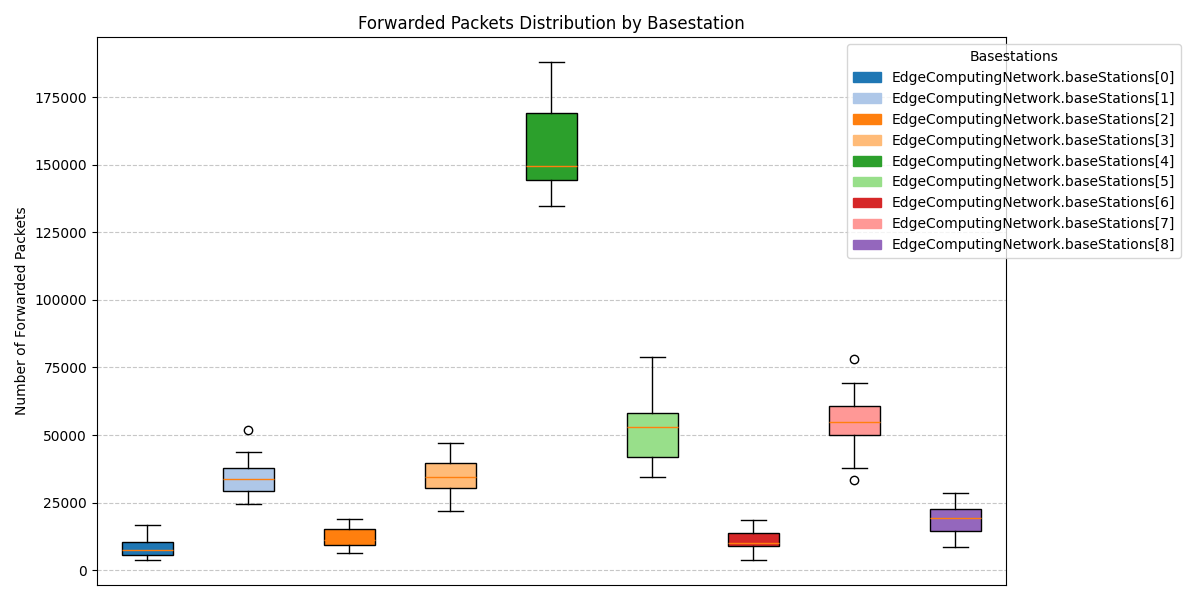
\includegraphics[width=\textwidth]{img/plots/log_1e4_B/forwarded.png}
    \caption{Forwarded packets distribution (lognormal)}
\end{figure}

\begin{figure}[H]
    \centering
    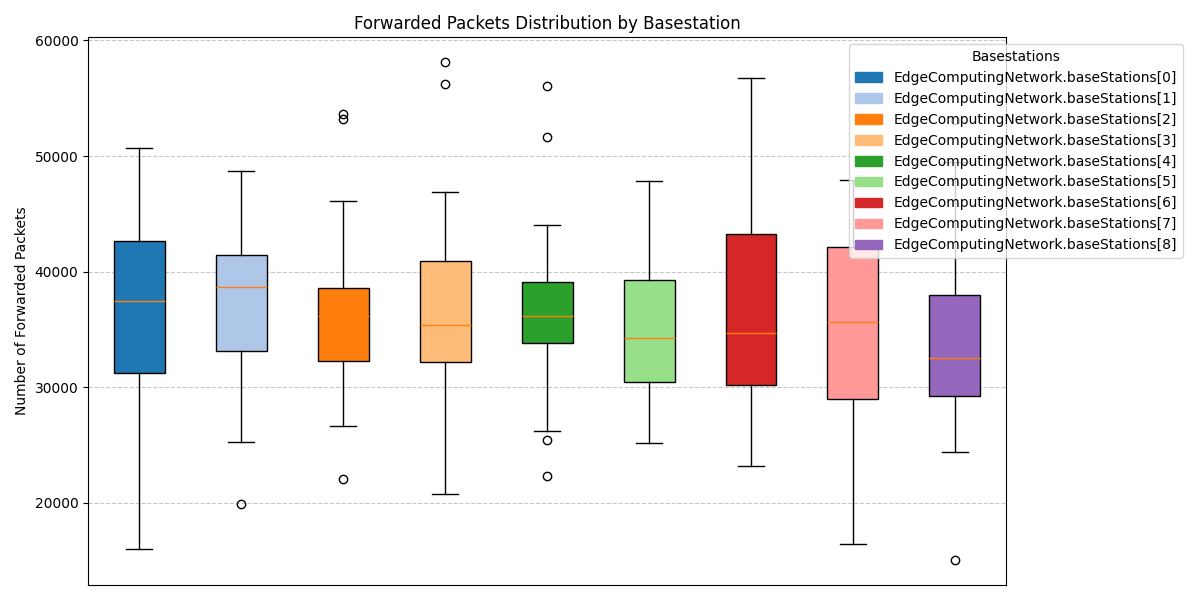
\includegraphics[width=\textwidth]{img/plots/uni_1e4_B/forwarded.png}
    \caption{Forwarded packets distribution (uniform)}
\end{figure}

\begin{flushleft}
It is shown the same behaviour as in the method A, the only difference is that in the uniform case packets are forwarded more evenly among all the base stations.
\vspace{1em}

We report a total of $9.7\times10^6$ forwarded packets for the uniform and $11.4\times10^6$ for the lognormal.
\end{flushleft}

\begin{figure}[H]
    \centering
    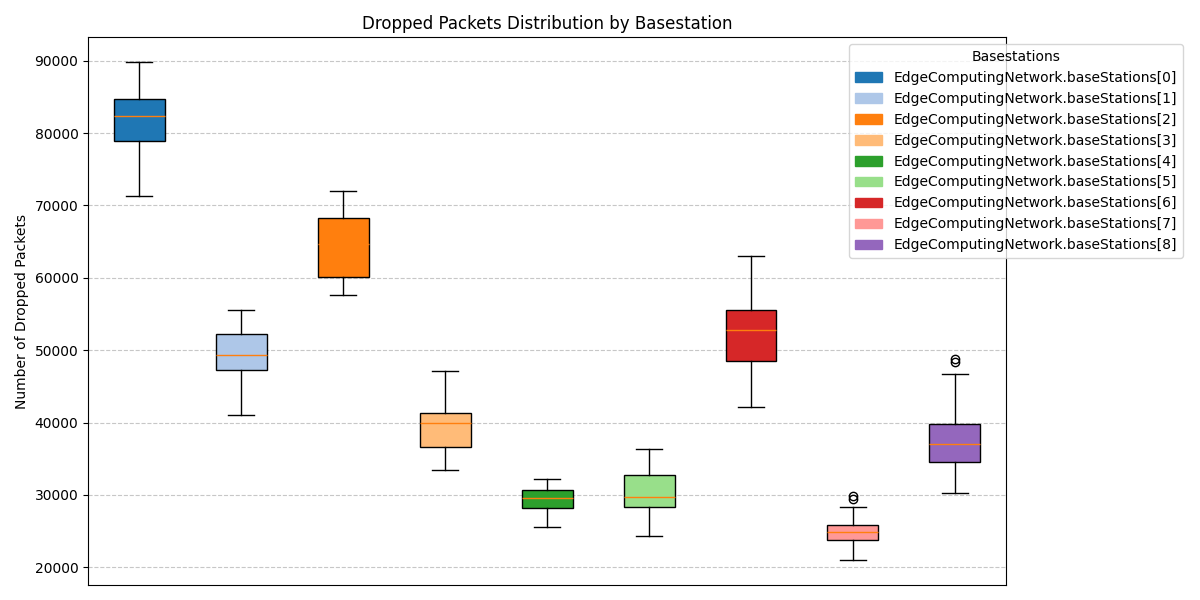
\includegraphics[width=\textwidth]{img/plots/log_1e4_B/dropped.png}
    \caption{Dropped packets distribution (lognormal)}
\end{figure}

\begin{figure}[H]
    \centering
    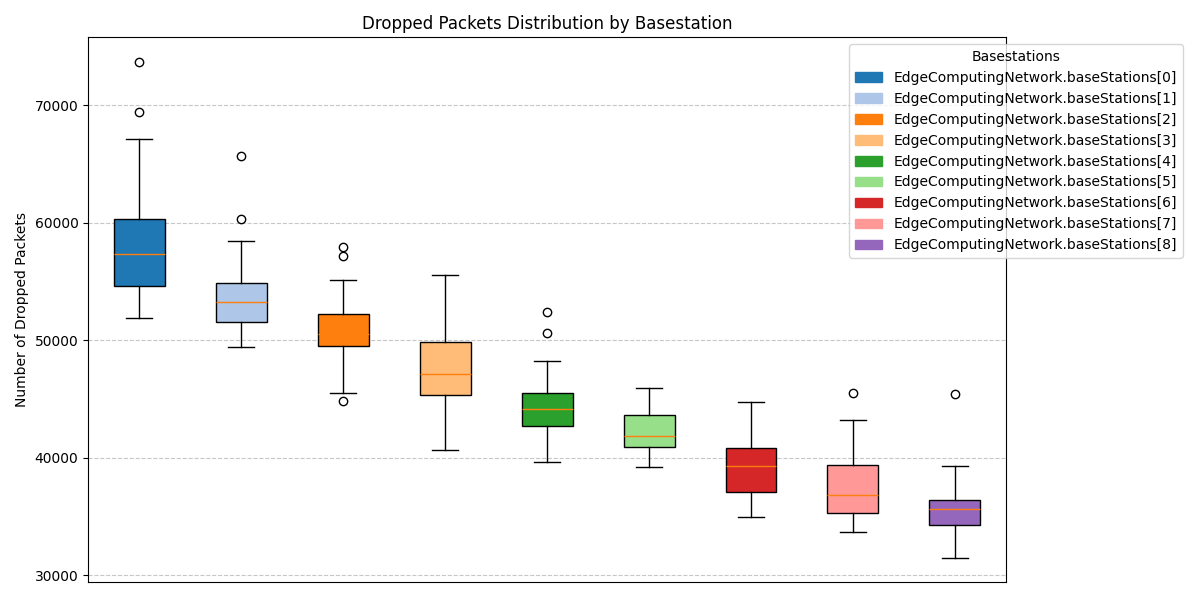
\includegraphics[width=\textwidth]{img/plots/uni_1e4_B/dropped.png}
    \caption{Dropped packets distribution (uniform)}
\end{figure}

\begin{flushleft}
As we can expect base stations that forward the majority of the packets are the ones that discard few of them and vice versa. We encounter this phenomenon for both the distributions.
\vspace{1em}

We report the same number of discarded packets both for the lognormal and the uniform distribution.
\end{flushleft}

% UNI
% Total Dropped Packets: 12284013
% Total Forwarded Packets: 9762424
% LOG
% Total Dropped Packets: 12285154
% Total Forwarded Packets: 11440655

\chapter{Conclusion}
\appendix
\end{document}